\section{Employees}

\subsection{TVS Motors employee force and diversity}

TVS Motor Company is committed to fostering a diverse and inclusive workforce, reflecting its core values and corporate culture. As of the latest reporting, the company employs over 25,000 people across its operations. Notably, women represent approximately 12\% \cite{TVS_ANNUAL_REPORT} of the overall workforce, which highlights TVS's commitment to promoting gender diversity in a traditionally male-dominated industry. The company has received accolades for its efforts in creating a supportive work environment, being recognized as one of the “Best Companies for Women” in India.

TVS Motor also prioritizes inclusivity by ensuring equal opportunities for all employees, including Persons with Disabilities (PwDs), who make up about 2\% of the workforce. The company implements various initiatives aimed at enhancing workplace diversity, such as on-campus childcare facilities, industry-leading maternity and paternity policies, and flexible working hours. These measures underscore TVS's dedication to creating an equitable workplace that values diverse perspectives and fosters an environment where all employees can thrive.

The detailed counts are found below:\\
(Employees are Skilled and Workers are unskilled) \\[1cm]
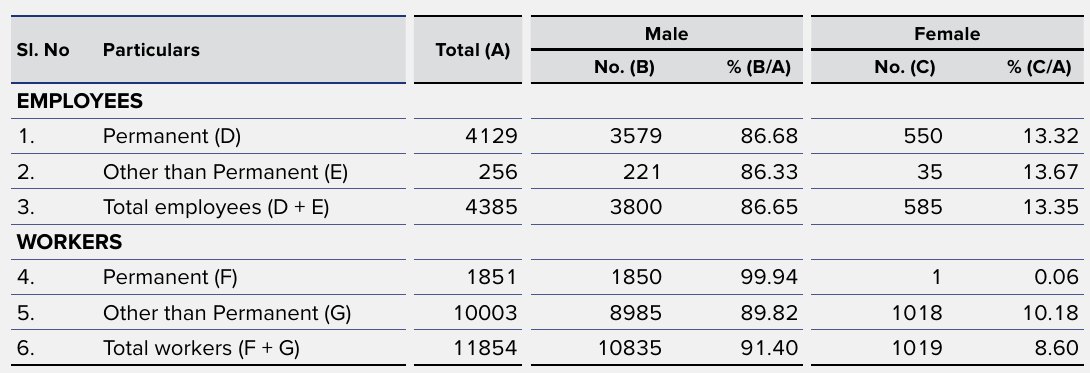
\includegraphics[width=\linewidth]{psycho_images/TVS_employee.png}

\subsection{Hero MotoCorp employee force and diversity}

Hero MotoCorp employs a total of approximately 30,000 individuals, comprising both permanent employees and workers\cite{hero_sreport}\cite{hero-rep}. The breakdown shows that there are about 4,534 permanent employees and 25,404 workers, with a significant representation of male employees (approximately 90.32\% of permanent employees and 91.58\% of workers).

In terms of diversity, the company is committed to promoting gender inclusion within its workforce. Currently, women represent about 9.68\% of permanent employees and 8.42\% of workers\cite{hero-rep}. Hero MotoCorp has set a goal to increase female representation to 30\% by 2030, reflecting its dedication to enhancing diversity and inclusion across all levels of the organization\cite{hero_sreport}. Additionally, the company actively engages in initiatives aimed at empowering women and supporting a diverse workplace, underscoring its commitment to fostering a more equitable work environment.

The details of the counts can be found below:\\
(Employees are Skilled and Workers are unskilled)
\begin{figure}[h]
	\subfloat{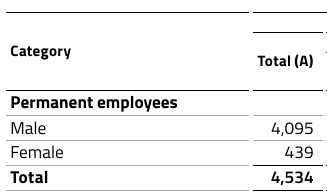
\includegraphics[width=0.5\linewidth]{psycho_images/Hero_employee_0.png}}
	\subfloat{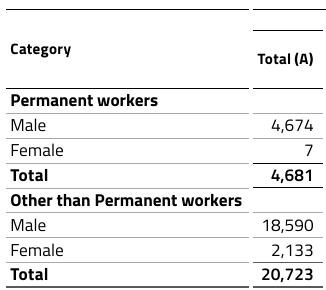
\includegraphics[width=0.5\linewidth]{psycho_images/Hero_employee_1.png}}
\end{figure}
